% SC4022 --- Chapter 5: Scale-Free & Preferential Attachment (0->100 ground-up)
\chapter{Scale-Free Networks \& Preferential Attachment}
\label{ch:scalefree}
\sloppy

\begin{quote}
\emph{``The rich get richer.''} --- In citation, Web, and social networks a few hubs hold most links while most nodes have few. This heavy tail is not Poisson noise; it follows a power law born from growth with preference.
\end{quote}

\noindent\fbox{\parbox{\dimexpr\linewidth-2\fboxsep-2\fboxrule}{%
\textbf{From zero: we build here, no power-law background needed.} We assume only Ch.~1 (degree distribution) and Ch.~4 (ER, configuration) plus basic probability. Power laws are introduced by picture, then defined, then derived via a generative mechanism.}}
\vspace{0.4em}

\section*{Learning Outcomes}
After this chapter you will be able to:
\begin{enumerate}[label=(L\arabic*)]
    \item recognise heavy-tailed degree distributions and plot them on log--log axes;
    \item define a power law $P(k)\sim k^{-\gamma}$, estimate $\gamma$ via MLE, and state its cutoff;
    \item derive the Barab\'asi--Albert model and show it yields $P(k)\sim k^{-3}$;
    \item simulate BA growth, measure hubs, exponent, and age--degree correlation;
    \item apply the Clauset--Shalizi--Newman test to critique scale-free claims.
\end{enumerate}

% ============================================================
\section{Heavy Tails and Power Laws}
\label{sec:heavy-tails}
\paragraph{Intuition.} In an ER graph with $\langle k\rangle=6$, seeing a node with $k=30$ is astronomically unlikely (Poisson tail $\sim e^{-k}$). Yet the Web has pages with millions of in-links while most have a handful. Plotting $P(k)$ on log--log axes turns an exponential into a curve but a power law into a straight line---a visual tell.

\begin{definition}[Power-law degree distribution]\label{def:powerlaw}
A distribution is (asymptotically) power-law if for $k\ge k_{\min}$,
\begin{equation}
P(k)=C\,k^{-\gamma},\qquad C=(\gamma-1)k_{\min}^{\,\gamma-1},
\end{equation}
with \emph{exponent} $\gamma>1$. On log--log, $\log P(k)=\log C-\gamma\log k$ is linear with slope $-\gamma$. Most real ``scale-free'' networks report $2<\gamma<3$, where $\langle k\rangle$ is finite but $\langle k^2\rangle$ diverges as $k_{\max}\to\infty$ (variance explodes---hubs dominate).
\end{definition}

Why care about $\gamma$? If $2<\gamma<3$, the second moment $\langle k^2\rangle$ grows with system size, which (Ch.~6--7) drives epidemic thresholds to zero and makes random removal harmless but hub targeting devastating.

\begin{figure}[h]\centering
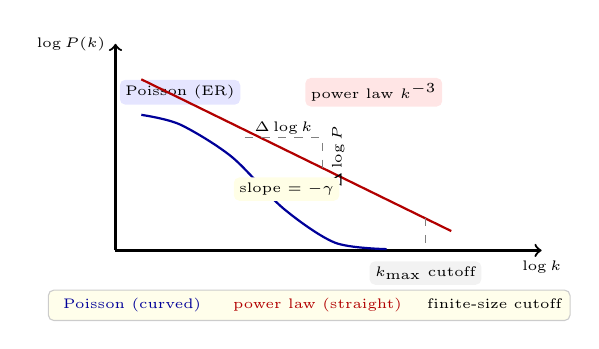
\begin{tikzpicture}[scale=0.82,every node/.style={font=\scriptsize}]
\draw[->,thick] (0,0)--(6.6,0) node[below,font=\tiny] {$\log k$};
\draw[->,thick] (0,0)--(0,3.2) node[left,font=\tiny] {$\log P(k)$};
% Poisson (curved)
\draw[thick,blue!60!black,smooth] plot coordinates {(0.4,2.1) (1.0,1.95) (1.8,1.45) (2.6,0.65) (3.4,0.12) (4.2,0.02)};
\node[font=\tiny,fill=blue!10,rounded corners=2pt,inner sep=2pt] at (1.0,2.45) {Poisson (ER)};
% Power law (straight)
\draw[thick,red!70!black] (0.4,2.65)--(5.2,0.30);
\node[font=\tiny,fill=red!10,rounded corners=2pt,inner sep=2pt] at (4.0,2.45) {power law $k^{-3}$};
% slope triangle
\draw[thin,gray,dashed] (2.0,1.75)--(3.2,1.75)--(3.2,1.15);
\node[font=\tiny] at (2.6,1.90) {$\Delta\log k$};
\node[font=\tiny,rotate=90] at (3.45,1.45) {$\Delta\log P$};
\node[font=\tiny,fill=yellow!10,rounded corners=2pt,inner sep=2pt] at (2.65,0.95) {slope $=-\gamma$};
% cutoff annotation
\draw[thin,gray,dashed] (4.8,0.50)--(4.8,0);
\node[font=\tiny,fill=gray!10,rounded corners=2pt,inner sep=2pt] at (4.8,-0.35) {$k_{\max}$ cutoff};
\node[font=\tiny,draw=gray!40,fill=yellow!8,rounded corners=2pt,inner sep=3pt] at (3.0,-0.85) {\textcolor{blue!60!black}{$\blacksquare$ Poisson (curved)} \quad \textcolor{red!70!black}{$\blacksquare$ power law (straight)} \quad finite-size cutoff};
\end{tikzpicture}
\caption{Log--log degree distribution. ER (Poisson) curves sharply down (blue); a power law $P(k)\sim k^{-\gamma}$ is a straight line with slope $-\gamma$ (red). Finite networks cut off at $k_{\max}$.}
\label{fig:powerlaw-loglog}
\end{figure}

\paragraph{Estimating $\gamma$.} Do not fit a line by least squares on the log--log histogram---it is biased. The maximum-likelihood estimator for continuous $k\ge k_{\min}$ is $\hat\gamma=1+n[\sum_i\ln(k_i/k_{\min})]^{-1}$ (Newman, 2005). Choose $k_{\min}$ by minimising the Kolmogorov--Smirnov distance between data and fitted power law. Then test goodness-of-fit (see \S\ref{sec:clauset}).

% ============================================================
\section{Barab\'asi--Albert Model}
\label{sec:ba-model}
\paragraph{Intuition.} Two ingredients make a power law: \emph{growth} (new nodes keep arriving) and \emph{preferential attachment} (newcomers prefer to link to already-popular nodes). ``When a new Web page appears, it is more likely to link to Google than to a personal homepage.'' The rich get richer.

\begin{definition}[Barab\'asi--Albert model]\label{def:ba}
Start with $m_0$ connected nodes. At each step add one new node with $m\le m_0$ edges, each attached to an existing node $i$ with probability
\begin{equation}
\Pi(k_i)=\frac{k_i}{\sum_j k_j}.
\end{equation}
After $t$ steps, $n=m_0+t$, $m=m_0(m_0-1)/2+mt$, and $\langle k\rangle=2m$.
\end{definition}

\begin{figure}[h]\centering
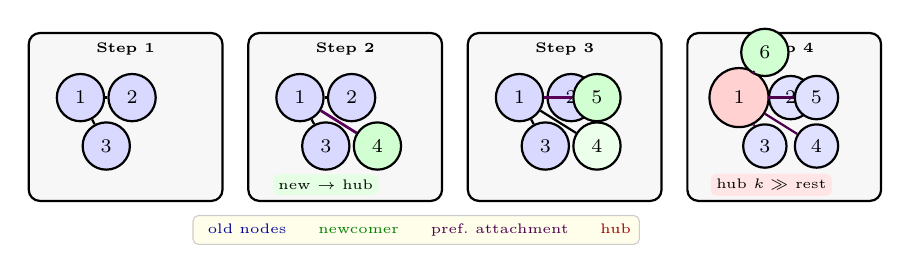
\begin{tikzpicture}[scale=0.82,every node/.style={font=\scriptsize}]
\foreach \step/\x in {1/0,2/3.4,3/6.8,4/10.2} {
\begin{scope}[xshift=\x cm]
\draw[thick,rounded corners=4pt,fill=gray!6] (-0.2,-0.6) rectangle (2.8,2.0);
\node[font=\tiny\bfseries] at (1.3,1.75) {Step \step};
\end{scope}}
% step 1: 3 nodes
\node[circle,draw,thick,fill=blue!15,minimum size=0.6cm] (a1) at (0.6,1.0) {1};
\node[circle,draw,thick,fill=blue!15,minimum size=0.6cm] (a2) at (1.4,1.0) {2};
\node[circle,draw,thick,fill=blue!15,minimum size=0.6cm] (a3) at (1.0,0.25) {3};
\draw[thick] (a1)--(a2); \draw[thick] (a1)--(a3);
% step 2: new node 4 attaches to 1 (hub)
\node[circle,draw,thick,fill=blue!15,minimum size=0.6cm] (b1) at (4.0,1.0) {1};
\node[circle,draw,thick,fill=blue!15,minimum size=0.6cm] (b2) at (4.8,1.0) {2};
\node[circle,draw,thick,fill=blue!15,minimum size=0.6cm] (b3) at (4.4,0.25) {3};
\node[circle,draw,thick,fill=green!18,minimum size=0.6cm] (b4) at (5.2,0.25) {4};
\draw[thick] (b1)--(b2); \draw[thick] (b1)--(b3); \draw[thick,violet!70!black,line width=1.0pt] (b4)--(b1);
\node[font=\tiny,fill=green!10,rounded corners=2pt,inner sep=2pt] at (4.4,-0.35) {new $\to$ hub};
% step 3
\node[circle,draw,thick,fill=blue!15,minimum size=0.6cm] (c1) at (7.4,1.0) {1};
\node[circle,draw,thick,fill=blue!15,minimum size=0.6cm] (c2) at (8.2,1.0) {2};
\node[circle,draw,thick,fill=blue!15,minimum size=0.6cm] (c3) at (7.8,0.25) {3};
\node[circle,draw,thick,fill=green!8,minimum size=0.6cm] (c4) at (8.6,0.25) {4};
\node[circle,draw,thick,fill=green!18,minimum size=0.6cm] (c5) at (8.6,1.0) {5};
\draw[thick] (c1)--(c2); \draw[thick] (c1)--(c3); \draw[thick] (c4)--(c1); \draw[thick,violet!70!black,line width=1.0pt] (c5)--(c1);
% step 4: hub dominates
\node[circle,draw,thick,fill=red!18,minimum size=0.75cm] (d1) at (10.8,1.0) {1};
\node[circle,draw,thick,fill=blue!12,minimum size=0.55cm] (d2) at (11.6,1.0) {2};
\node[circle,draw,thick,fill=blue!12,minimum size=0.55cm] (d3) at (11.2,0.25) {3};
\node[circle,draw,thick,fill=blue!12,minimum size=0.55cm] (d4) at (12.0,0.25) {4};
\node[circle,draw,thick,fill=blue!12,minimum size=0.55cm] (d5) at (12.0,1.0) {5};
\node[circle,draw,thick,fill=green!18,minimum size=0.6cm] (d6) at (11.2,1.7) {6};
\foreach \v in {d2,d3,d4,d5,d6} \draw[thick,violet!60!black] (d1)--(\v);
\node[font=\tiny,fill=red!10,rounded corners=2pt,inner sep=2pt] at (11.3,-0.35) {hub $k\gg$ rest};
\node[font=\tiny,draw=gray!40,fill=yellow!8,rounded corners=2pt,inner sep=3pt] at (5.8,-1.05) {\textcolor{blue!60!black}{$\blacksquare$ old nodes} \quad \textcolor{green!50!black}{$\blacksquare$ newcomer} \quad \textcolor{violet!60!black}{$\blacksquare$ pref.\ attachment} \quad \textcolor{red!60!black}{$\blacksquare$ hub}};
\end{tikzpicture}
\caption{BA growth: each new node (green) attaches preferentially to high-degree nodes (violet edges). Early nodes accumulate links and become hubs (red). After many steps, $P(k)\sim k^{-3}$.}
\label{fig:ba-growth}
\end{figure}

\begin{theorem}[BA exponent]\label{thm:ba-exponent}
In the BA model with $m$ edges per new node, the stationary degree distribution is $P(k)=2m(m+1)/[k(k+1)(k+2)]\sim2m^2k^{-3}$ for $k\ge m$, so $\gamma=3$ universally (continuum theory: $k_i(t)=m\sqrt{t/t_i}$ where $t_i$ is birth time).
\end{theorem}
\begin{proof}[Sketch]
Continuum approximation: treat $k_i$ as continuous, $dk_i/dt=m\Pi(k_i)=mk_i/(2mt)=k_i/(2t)$ since $\sum_jk_j=2mt$. Solve: $dk_i/k_i=dt/(2t)$, so $k_i(t)=m(t/t_i)^{1/2}$. The fraction of nodes with $k_i(t)>k$ equals $\Pr(t_i<t(m/k)^2)=1-(m/k)^2$, differentiate to get $P(k)=2m^2k^{-3}$. The master-equation proof yields the exact form. \qed
\end{proof}

Consequences: age correlates with degree (old nodes are hubs), $k_{\max}\sim m\sqrt{n}$, and the exponent $3$ is robust---but variants change it (fitness, nonlinear attachment, copying).

\begin{figure}[h]\centering
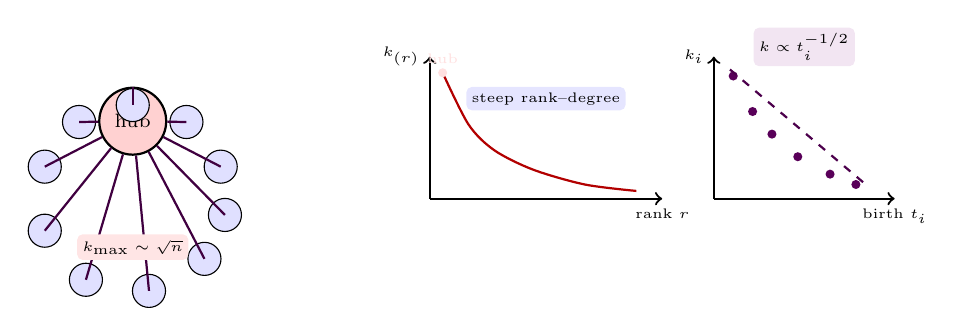
\begin{tikzpicture}[scale=0.82,every node/.style={font=\scriptsize}]
% hub-and-spoke drawing
\node[circle,draw,thick,fill=red!18,minimum size=0.85cm] (hub) at (0,1.2) {hub};
\foreach \a in {20,55,90,125,160,200,240,280,320,350} {\node[circle,fill=blue!12,draw,minimum size=0.42cm] at (\a:1.45) {}; \draw[thick,violet!50!black] (hub)--(\a:1.45);}
\node[font=\tiny,fill=red!10,rounded corners=2pt,inner sep=2pt] at (0,-0.75) {$k_{\max}\sim\sqrt{n}$};
% degree rank plot
\begin{scope}[xshift=4.6cm]
\draw[->,thick] (0,0)--(3.6,0) node[below,font=\tiny] {rank $r$};
\draw[->,thick] (0,0)--(0,2.2) node[left,font=\tiny] {$k_{(r)}$};
\draw[thick,red!70!black,smooth] plot coordinates {(0.2,1.95) (0.6,1.15) (1.0,0.75) (1.6,0.45) (2.4,0.22) (3.2,0.12)};
\fill[red!12] (0.2,1.95) circle (2pt) node[above,font=\tiny] {hub};
\node[font=\tiny,fill=blue!10,rounded corners=2pt,inner sep=2pt] at (1.8,1.55) {steep rank--degree};
\end{scope}
% age vs degree
\begin{scope}[xshift=9.0cm]
\draw[->,thick] (0,0)--(2.8,0) node[below,font=\tiny] {birth $t_i$};
\draw[->,thick] (0,0)--(0,2.2) node[left,font=\tiny] {$k_i$};
\foreach \x/\y in {0.3/1.9,0.6/1.35,0.9/1.0,1.3/0.65,1.8/0.38,2.2/0.22} \fill[violet!70!black] (\x,\y) circle (2pt);
\draw[thick,violet!60!black,dashed] (0.25,2.0)--(2.4,0.18);
\node[font=\tiny,fill=violet!10,rounded corners=2pt,inner sep=2pt] at (1.4,2.35) {$k\propto t_i^{-1/2}$};
\end{scope}
\end{tikzpicture}
\caption{Left: BA hub-and-spoke. Middle: rank--degree is steep (few hubs, many leaves). Right: older nodes have larger degree---a testable age--degree correlation.}
\label{fig:ba-hub}
\end{figure}

% ============================================================
\section{Critiquing Scale-Free Claims}
\label{sec:clauset}
\paragraph{Intuition.} Many papers claim ``our network is scale-free'' after eyeballing a straight line on log--log. Clauset, Shalizi, and Newman (2009) showed that rigorous testing rejects most such claims---exponentials, log-normals, and truncated power laws often fit better.

The recipe: (i) estimate $k_{\min}$ and $\gamma$ by MLE, (ii) compute KS statistic $D$ for goodness-of-fit, (iii) generate synthetic power-law datasets with same $n$, $k_{\min}$, $\gamma$ and compare $D$---a $p$-value below $0.1$ rejects the power-law hypothesis. Even when not rejected, compare against alternatives via likelihood-ratio (Vuong) test. The configuration model with power-law $P(k)$ can then serve as a null for dynamics (Ch.~6--7).

\begin{lstlisting}[language=Python, caption={BA simulation: growth, exponent, and age--degree correlation.}, label={lst:ba-sim}]
import networkx as nx
import numpy as np

G = nx.barabasi_albert_graph(500, 3, seed=0)
degrees = np.array([d for _, d in G.degree()])
print(f"n=500 m=3 <k>={degrees.mean():.1f} max k={degrees.max()}")

# Log-log degree histogram (check straight line)
import collections
cnt = collections.Counter(degrees)
ks, pk = zip(*sorted(cnt.items()))
# MLE for gamma (continuous approx, k_min=3)
k_min = 3
tail = degrees[degrees >= k_min]
gamma_hat = 1 + len(tail) / np.sum(np.log(tail / k_min))
print(f"MLE gamma ~ {gamma_hat:.2f} (BA predicts 3.0)")

# Age-degree: node id is birth order in NetworkX BA
import matplotlib.pyplot as plt
# Hub age check: oldest nodes should have highest degree
top5 = sorted(G.degree, key=lambda x: x[1], reverse=True)[:5]
print("top hubs (node, k, birth):", [(v, k, v) for v,k in top5])
\end{lstlisting}

\begin{lstlisting}[language=Python, caption={PLFit and Clauset test sketch: is this really a power law?}, label={lst:plfit}]
import networkx as nx
import numpy as np

# Compare Poisson (ER) vs power-law (BA) tail likelihood
ER = nx.erdos_renyi_graph(500, 0.012, seed=1)
BA = nx.barabasi_albert_graph(500, 3, seed=1)
for name, G in [("ER", ER), ("BA", BA)]:
    degs = np.array([d for _, d in G.degree()])
    # Simple tail check: fraction with k > 2<k>
    frac = (degs > 2*degs.mean()).mean()
    print(f"{name}: <k>={degs.mean():.1f} P(k>2<k>)={frac:.3f}"
          f" max={degs.max()}")
# ER tail fraction ~ Poisson (tiny); BA tail heavy (large)
# For rigorous test use `powerlaw` package: powerlaw.Fit(degs)
\end{lstlisting}

% ============================================================
\section{Chapter Notes}
Price (1965) first modelled cumulative advantage for citations; Barab\'asi and Albert (1999, \emph{Science}) popularised preferential attachment for networks. The exact $P(k)\sim k^{-3}$ solution is due to Krapivsky et~al. and Dorogovtsev--Mendes. Variants (Bianconi--Barab\'asi fitness, copying, redirection, nonlinear $\Pi\sim k^\alpha$) tune $\gamma$ or break scale-free entirely. Clauset et~al.\ (2009) and Broido \& Clauset (2019) provide the modern statistical critique---``scale-free networks are rare'' when tested rigorously.

% ============================================================
\section{Exercises}
\label{sec:ch05-exercises}
\begin{enumerate}[label=E5.\arabic*, leftmargin=*, itemsep=0.8em]
    \item \textbf{Log--log by hand.} Given degrees $[1,1,1,2,2,5,9,14]$, plot $P(k)$ vs $k$ on log--log (sketch). Does a Poisson or power law seem more plausible? Estimate $\gamma$ crudely from the slope between $k=2$ and $k=14$.
    \item \textbf{Continuum derivation.} Starting from $dk_i/dt=k_i/(2t)$, $k_i(t_i)=m$, integrate to get $k_i(t)=m\sqrt{t/t_i}$. Then show $\Pr(k_i(t)>k)=(m/k)^2$ and differentiate to obtain $P(k)\sim k^{-3}$.
    \item \textbf{Simulate and measure.} Generate BA($n=1000$, $m=2$) and compute degree histogram. Fit $\gamma$ via MLE with $k_{\min}=m$ and report. Does doubling $m$ change $\hat\gamma$? Explain.
    \item \textbf{Age--degree.} In your BA graph, compute Pearson correlation between node birth time (id) and final degree. Is it negative as predicted? Compare with an ER graph of same $n$, $\langle k\rangle$.
    \item \textbf{Clauset test.} Use the `powerlaw` package (or hand KS) to test whether a BA($500,3$) degree sequence is plausibly power-law ($p>0.1$) and whether an ER($500,0.012$) sequence is rejected. Report $k_{\min}$, $\hat\gamma$, and $p$-values.
\end{enumerate}
% End of Chapter 5
